% !Mode:: "TeX:UTF-8"
% Translator: Yujun Li 
\chapter{实用方法}
\label{chap:practical_methodology}
对于一个优秀的机器学习实践者而言,成功地使用深度学习技术,不仅仅需要知道存在哪些算法和算法原理,还需要知道如何针对具体应用挑选一个合适的算法,以及如何监控,并根据实验反馈改进机器学习系统。
在\gls{ML}系统的日常开发中,实践者需要决定是否收集更多的数据,增加或减少模型容量,添加或删除正则化功能,改进模型的优化,改进模型的近似推断,或调试模型的软件实现。
尝试这些操作都需要大量时间,因此确定正确做法,而不盲目猜测是尤为重要的。

本书的大部分内容都是关于不同的\gls{ML}模型,训练算法和目标函数。
这可能给人一种印象,成为\gls{ML}专家的最重要因素是了解各种各样的\gls{ML}技术,熟悉各种不同的数学。
在实践中,正确使用一个普通算法通常比草率使用一个不确定的算法效果更好。
正确应用一个算法需要掌握一些相当简单的方法。
本章的许多建议都来自\cite{ng-lecture-advice}。

我们建议实践中参考以下几个设计流程:
\begin{itemize}
\item 确定目标——使用什么\gls{error_metric},并为此\gls{error_metric}指定目标值。
这些目标和\gls{error_metric}应受驱动于该应用旨在解决的问题。

% -- 409 --

\item 尽快建立一个\gls{end_to_end}的工作流程,包括合适的\gls{performance_metrics}的估计。

\item 搭建系统,确定性能瓶颈。
检查哪个部分的性能差于预期,以及是否是因为过拟合,欠拟合,或者数据或软件缺陷造成的。

\item 根据具体观察重复逐步改动,如收集新数据,调整\gls{hyperparameter},或改进算法。
\end{itemize}

我们将使用街景地址号码\gls{transcription_system}\citep{Goodfellow+et+al-ICLR2014a}作为一个正在运行的示例。
该应用的目标是添加建筑物到谷歌地图。
街景车拍摄建筑物,并记录与每张建筑照片相关的GPS坐标。
\gls{CNN}识别每张照片上的地址号码,由谷歌地图数据库在正确的位置添加该地址。
这个商业应用如何开发的流程是一个很好的如何遵循我们倡导的设计方法的示例。

我们现在描述这个过程中的每一个步骤。

\section{\glsentrytext{performance_metrics}}
\label{sec:performance_metrics}
确定目标,即使用什么\gls{error_metric},是必要的第一步,因为\gls{error_metric}将指导接下来的所有工作。
同时我们也应该了解大概能得到什么级别的目标性能。

注意,对于大多数应用而言,不可能实现绝对零误差。
即使你有无限的训练数据,并且恢复了真正的\gls{PD},\gls{bayes_error}仍定义了能达到的最小\gls{error_rate}。
这是因为输入特征可能无法包含输出变量的完整信息,或是因为系统可能本质上是随机的。
当然我们还会受限于有限的训练数据。

训练数据的数量会因为各种原因受到限制。
当目标是打造现实世界中最好的产品或服务时,通常需要收集更多的数据,但必须确定进一步减少误差的价值,并与收集更多数据的成本做权衡。
数据收集会耗费时间,金钱,或带来痛苦(例如,收集人体医疗测试数据)。
科研中,目标通常是在某个确定\gls{benchmarks}下探讨哪个算法更好,一般会固定训练集,不能收集更多的数据。

% -- 410 --

如何确定合理的性能期望?
在学术界,通常我们可以根据先前公布的\gls{benchmarks}结果来估计预期\gls{error_rate}。
在现实世界中,一个应用的\gls{error_rate}有必要是安全的,具有成本效益的,或吸引消费者的。
一旦你确定了想要达到的\gls{error_rate},那么你的设计将由如何达到这个\gls{error_rate}来指导。

除了需要考虑\gls{performance_metrics}之外,另一个需要考虑的是度量的选择。
我们有几种不同的\gls{performance_metrics},可以用来度量含有\gls{ML}的应用的性能。
这些\gls{performance_metrics}通常不同于训练模型的损失函数。 
如\secref{sec:the_performance_measure_p}所述,我们通常会度量一个系统的\gls{accuracy},或等价的\gls{error_rate}。

然而,许多应用需要更高级的度量。

有时,一种错误可能会比更一种错误更严重。
例如,垃圾邮件检测系统会有两种错误:将正常邮件归为垃圾邮件,将垃圾邮件归为正常邮件。
阻止正常消息比通过可疑消息更糟糕。
不去度量垃圾邮件分类的\gls{error_rate},我们希望度量某种形式的总损失,其中拦截正常邮件比通过垃圾邮件的代价更高。

有时,我们需要训练检测某些罕见事件的二元分类器。
例如,我们可能会为一种罕见疾病设计医疗测试。
假设每一百万人中只有一人患病。
简单地让分类器一直报告没有患者,我们就能在检测任务上实现$99.9999\%$的正确率。
显然,正确率很差地体现了这种系统的性能。
解决这个问题的方法是度量\firstgls{precision}和\firstgls{recall}。
\gls{precision}是模型报告的检测是正确的比率,而\gls{recall}则是真实事件被检测到的比率。
检测器一只报告没有患者,可能会有一个很高的\gls{precision},但\gls{recall}为零。
而报告每个人都是患者的检测器可能有很高的\gls{recall},但是\gls{precision}很低(在我们的例子是$0.0001\%$,每一百万人只有一人患病)。
当使用\gls{precision}和\gls{recall}时,通常会画\textbf{PR曲线},y轴表示\gls{precision},x轴表示\gls{recall}。
如果检测到的事件发生了,那么分类器会返回一个比较高的值。
例如,我们将\gls{feedforward_network}设计为检测一种疾病,估计一个医疗结果由特征$\Vx$表示的人患病的概率为$\hat{y} = P(y=1\mid\Vx)$。
每当这个值超过某个阈值时,我们报告检测结果。
通过调整阈值,我们能以\gls{precision}换\gls{recall}。
在很多情况下,我们希望用一个数而不是曲线来概括分类器的性能。
要做到这一点,我们可以转换\gls{precision} $p$和\gls{recall} $r$为\textbf{F-score}
\begin{equation}
	F = \frac{2pr}{p+r}.
\end{equation}
另一种方法是报告PR曲线下方的总面积。

% -- 411 --

在一些应用中,\gls{ML}系统可能会拒绝做出判断。
\gls{ML}算法能够估计对判断的确信度,会是非常有用的,特别是在错误判断会有严重危害,而人工操作员能够偶尔接管的情况下。
街景\gls{transcription_system}可以作为这种情况的一个示例。
该任务是转录照片上的地址号码,以关联到地图上拍摄照片的位置。
因为如果地图是不精确的,那么地图的价值会严重下降。
因此只在转录正确的情况下添加地址十分重要。
如果\gls{ML}系统认为它不太能像人一样正确地转录,那么最好办法当然是让人来转录照片。
当然,我们有必要让\gls{ML}系统大量降低需要人工操作处理的图片,这样它才是有用的。
在这种情况下,一种自然的\gls{performance_measures}是\firstgls{coverage}。
\gls{coverage}是\gls{ML}系统能够产生响应的样本所占的比率。
有可能以\gls{coverage}换\gls{precision}。
一个系统总可以通过拒绝处理任意样本的方式来达到$100\%$的\gls{precision},但是\gls{coverage}降到了$0\%$。
对于街景任务,该项目的目标是达到人类转录的\gls{precision},同时保持$95\%$的\gls{coverage}。
这项任务的人类级别性能是$98\%$的\gls{precision}。

还有许多其他的\gls{performance_measures}。
例如,我们可以度量点击率,收集用户满意度调查,等等。
许多专业的应用领域也有特定于应用的标准。

最重要的是首先要确定改进哪个\gls{performance_measures},然后集中提高\gls{performance_measures}。
如果没有明确的目标,那么我们很难判断\gls{ML}系统上的改动是否有所改进。

% -- 412 --

\section{默认的\glsentrytext{baseline}模型}
\label{sec:default_baseline_models}
确定\gls{performance_metrics}和目标后,任何实际应用的下一步是尽快建立一个合理的\gls{end_to_end}系统。

本节给出了一些建议,在不同情况下使用哪种算法作为第一个\gls{baseline}方法。

在本节中,我们提供了关于不同情况下使用哪种算法作为第一\gls{baseline}方法的建议。
值得注意的是,\gls{DL}研究进展迅速,所以本书出版后很快可能会有更好的默认算法。

根据问题的复杂性,项目开始时可能无需使用\gls{DL}。
如果可以只需正确选择几个线性权重来解决问题,那么项目可以开始于一个简单的统计模型,如\gls{logistic_regression}。

如果问题属于``\glssymbol{AI}-完成''类的,如\gls{object_recognition},\gls{SR},\gls{machine_translation},等等,那么项目开始于一个合适的\gls{DL}模型,效果会比较好。

首先,根据数据的结构选择一类合适的模型。
如果项目是以固定大小的向量作为输入的\gls{supervised_learning},那么可以使用全连接的\gls{feedforward_network}。
如果输入有已知的拓扑结构(例如,输入是图像),那么可以使用卷积网络。
在这些情况下,刚开始可以使用某种\gls{piecewise}线性单元(\glssymbol{ReLU}或者其扩展,如\glssymbol{leaky_ReLU},\glssymbol{PReLU}和\glssymbol{maxout})。
如果输入或输出是一个序列,可以使用\gls{gated_recurrent_net}(\glssymbol{LSTM}或\glssymbol{gated_recurrent_unit})。

具有衰减学习率动量的\glssymbol{SGD}是一个合理的优化算法选择
(流行的衰减方法有,衰减到固定最低学习率的线性衰减,指数衰减,或每次发生验证错误高原时降低学习率$2-10$倍,这些衰减方法在不同问题上好坏不一)。
另一个非常合理的选择是Adam算法。
\gls{batch_normalization}对优化性能有着显著的影响,特别是对卷积网络和具有\gls{sigmoid}非线性函数的网络而言。
虽然在最初的\gls{baseline}中忽略\gls{batch_normalization}是合理的,然而当优化似乎出现问题时,应该立刻使用\gls{batch_normalization}。

除非训练集包含数千万以上的样本,否则项目应该在一开始就包含一些简单的\gls{regularization}。 
\gls{early_stopping}也应该普遍采用。
\gls{dropout}也是一个很容易实现,且兼容很多模型和训练算法的良好\gls{regularizer}。
\gls{batch_normalization}有时也能降低\gls{generalization_error},并且因为标准化每个变量的统计估计而带来的\gls{noise},可以省略\gls{dropout}。

% -- 413 --

如果我们的任务和另一个被广泛研究的任务很相似,那么通过复制先前研究中已知性能良好的模型和算法,可能会得到很好的效果。
甚至可以从该任务中复制一个训练好的模型。
例如,通常会使用ImageNet上训练好的\gls{convolutional_network}的特征来解决其他计算机视觉问题\citep{girshickregion}。

一个常见问题是项目开始时是否使用\gls{unsupervised_learning},我们将在第三部分进一步探讨这个问题。
 这个问题和特定领域有关。
在某些领域,比如自然语言处理,能够在很大程度上受益于\gls{unsupervised_learning}技术,如学习无监督\gls{word_embeddings}。
在其他领域,如计算机视觉,除非是在\gls{semi_supervised}的设定下(有标签的样本数量很少)\citep{Kingma-et-al-NIPS2014,Rasmus-et-al-arxiv2015},目前\gls{unsupervised_learning}并没有带来益处。
如果应用所在环境中,\gls{unsupervised_learning}被认为是很重要的,那么将其包含在第一个\gls{end_to_end}\gls{baseline}中。
否则,只有在解决无监督问题时,才第一次尝试就使用\gls{unsupervised_learning}。
我们总能在之后发现初始\gls{baseline}过拟合的时候,加入\gls{unsupervised_learning}。

\section{是否收集更多数据}
\label{sec:determining_whether_to_gather_more_data}
在建立第一个\gls{end_to_end}系统后,就可以度量算法性能,改进算法。
许多\gls{ML}新手都忍不住尝试很多不同的算法来进行改进。
然而,往往收集更多的数据比改进学习算法要见效得多。

怎样判断是否要收集更多的数据?
首先,确定训练集上的性能是否可接受。
如果训练集上的性能差,学习算法还不能在训练集上学习出良好的模型,那么就没必要收集更多的数据。
反之,可以尝试增加更多的网络层或每层增加更多的\gls{hidden_unit},增加模型的规模。
此外,也可以尝试调整学习率等\gls{hyperparameter}来改进学习算法。
如果更大的模型和仔细调试的优化算法没有效果,那么问题可能源自训练数据的\emph{质量}。
数据可能含太多\gls{noise},或是可能不包含预测输出所需的正确输入。
这意味着需要重新开始,收集更干净的数据或是收集特征更丰富的数据集。

% -- 414 --

如果训练集上的性能是可接受的,那么度量测试集上的性能。
如果测试集上的性能也是可以接受的,那么就顺利完成了。
如果测试集上的性能比训练集的要差得多,那么收集更多的数据是最有效的解决方案之一。

这时主要的考虑是收集更多数据的代价和可行性,其他方法降低测试误差的代价和可行性,和增加数据数量能否显著提升测试集性能。
在拥有百万甚至上亿用户的大型网络公司,收集大型数据集是可行的,并且这样做的成本可能比其他方法要少很多,所以答案几乎总是收集更多的训练数据。
例如,收集大型带标签数据集是解决\gls{object_recognition}问题的主要因素之一。
在其他情况下,如医疗应用,收集更多的数据可能代价很高或者不可行。
一个替代收集更多数据的简单方法是降低模型规模或是改进\gls{regularization},如调整\gls{hyperparameter},如权重衰减系数,或是加入正则化策略,如\gls{dropout}。
如果调整\gls{regularization}\gls{hyperparameter}后,训练集性能和测试集性能之间的差距还是不可接受,那么收集更多的数据是可取的。

在决定是否收集更多的数据时,也需要确定收集多少数据。
如\figref{fig:chap5_training_size_grows}所示,绘制曲线显示训练集规模和\gls{generalization_error}之间的关系是很有帮助的。
根据走势延伸曲线,可以预测还需要多少训练数据来达到一定的性能。
通常,加入总数目一小部分的样本不会对\gls{generalization_error}产生显著的影响。
因此,建议在对数尺度上考虑训练集的大小,例如在新的实验上倍增样本数目。

如果收集更多的数据是不可行的,那么改进\gls{generalization_error}的唯一方法是改进学习算法本身。
这属于研究领域,并非对应用实践者的建议。

\section{选择\glsentrytext{hyperparameter}}
\label{sec:selecting_hyperparameters}
大部分\gls{DL}算法都有许多\gls{hyperparameter}来控制算法。
有些\gls{hyperparameter}会影响算法运行的时间和存储成本。
有些\gls{hyperparameter}会影响学习到的模型质量,以及在新输入上推断正确结果的能力。

% -- 415 --

有两种选择\gls{hyperparameter}的基本方法:手动选择和自动选择。
手动选择\gls{hyperparameter}需要了解\gls{hyperparameter}做了些什么,以及\gls{ML}模型如何取得良好的泛化。
自动选择\gls{hyperparameter}算法大大减少了解这些想法的需要,但它们往往需要更高的计算成本。

\subsection{手动调整\glsentrytext{hyperparameter}}
\label{sec:manual_hyperparameter_tuning}
手动设置\gls{hyperparameter},我们必须了解\gls{hyperparameter},训练误差,\gls{generalization_error}和计算资源(内存和运行时间)之间的关系。
这需要切实了解\chapref{chap:machine_learning_basics}学习算法的有效容量。

手动搜索\gls{hyperparameter}的目标通常是最小化受限于运行时间和内存预算的\gls{generalization_error}。
我们不去探讨如何确定各种\gls{hyperparameter}对运行时间和内存的影响,因为这高度依赖于平台。

手动搜索\gls{hyperparameter}的主要目标是调整模型的有效容量以匹配任务的复杂性。
有效容量受限于三个因素:模型的表示容量,学习算法成功最小化训练模型成本函数的能力,以及\gls{cost_function}和训练过程正则化模型的程度。
具有更多网络层,每层有更多\gls{hidden_unit}的模型具有较高的表达能力——能够表示更复杂的函数。
然而,如果训练算法不能找到合适的函数来最小化训练代价,或是如果\gls{regularization}项,如权重衰减,排除了这些函数,那么模型就不能学习到所有这些函数。

当\gls{generalization_error}以某个\gls{hyperparameter}为变量,作为函数绘制出来时,通常会表现为U形曲线,如\figref{fig:chap5_generalization_vs_capacity}所示。
在某个极端情况下,\gls{hyperparameter}对应着低容量,并且\gls{generalization_error}由于训练误差较大而很高。
这便是欠拟合的情况。
另一种极端情况,\gls{hyperparameter}对应着高容量,并且\gls{generalization_error}由于训练误差和测试误差之间的差距较大而很高。
最优的模型容量位于曲线中间的某个位置,能够达到最低可能的\gls{generalization_error},由中等的泛化误差和中等的训练误差相加构成。


% -- 416 --

\gls{hyperparameter}数值太大时,会发生过拟合。
例如,中间层\gls{hidden_unit}数量太大时,会发生过拟合。
因为\gls{hidden_unit}数量增多提高了模型\gls{capacity}。
\gls{hyperparameter}数值太小时,也会发生过拟合。
例如,权重衰减系数为零时,学习算法具有最大的有效容量,容易过拟合。

并非每个\gls{hyperparameter}都能对应着完整的U形曲线。
很多\gls{hyperparameter}是离散的,如中间层单元数目或是\gls{maxout_unit}中线性元件的数目,这种情况只能沿曲线探索离散的点。
有些\gls{hyperparameter}是二值的。
通常这些\gls{hyperparameter}用来指定是否使用学习算法中的一些可选部分,如预处理步骤减去均值,除以标准差,标准化输入特征。
这些\gls{hyperparameter}只能探索曲线上的两点。
其他一些\gls{hyperparameter}可能会限制其探索曲线某部分的最大值或最小值。
例如,权重衰减系数最小是零。
这意味着,如果权重衰减系数为零时模型欠拟合,那么我们将无法通过修改权重衰减系数探索过拟合区域。
换言之,有些\gls{hyperparameter}只能减少模型容量。

学习率可能是最重要的\gls{hyperparameter}。
如果你只有时间调整一个\gls{hyperparameter},那就调整学习率。
相比其他\gls{hyperparameter},它以一种更复杂的方式控制模型的有效容量——当学习率适合优化问题时,模型的有效容量最高,此时学习率既不是特别大也不是特别小。
学习率关于训练误差具有U形曲线,在\figref{fig:chap11_lr}所示。
当学习率过大时,梯度下降可能会不经意地增加而非减少训练误差。
在理想化的二次情况下,如果学习率是最佳值的两倍大时,会发生这种情况\citep{LeCun+98backprop-small}。
当学习率太小,训练不仅慢,还有可能永久停留在一个很高的训练误差。
关于这种情况,我们知之甚少(不会发生于一个凸损失函数中)。

\begin{figure}[!htb]
\ifOpenSource
\centerline{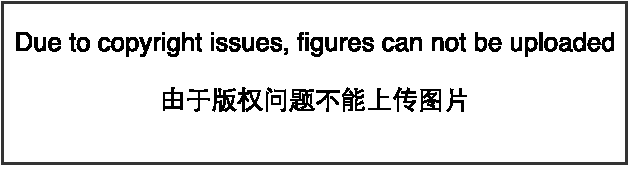
\includegraphics{figure.pdf}}
\else
\centerline{\includegraphics{Chapter11/figures/lr_color}}
\fi
\caption{\gls{training_error}和\gls{learning_rate}之间的典型关系。
要注意当\gls{learning_rate}大于最优值时误差会有显著的提升。
此图是对于固定的训练时间,越小的\gls{learning_rate}有时候可以以一个正比于\gls{learning_rate}减小量的因素来减慢训练过程。
\gls{generalization_error}也会得到类似的曲线,由于正则项作用在\gls{learning_rate}过大或过小处比较复杂。
由于一个糟糕的优化从某种程度上说可以避免\gls{overfitting},即使是\gls{training_error}相同的点也会拥有完全不同的\gls{generalization_error}。}
\label{fig:chap11_lr}
\end{figure}

调整学习率外的其他参数时,需要同时监测训练误差和测试误差,以判断您的模型是否过拟合或欠拟合,然后适当调整其容量。

如果训练集错误率大于目标\gls{error_rate},那么只能增加模型容量以改进模型。
如果没有使用\gls{regularization},并且确信优化算法正确运行,那么有必要添加更多的网络层或\gls{hidden_unit}。
然而,令人遗憾的是,这增加了模型的计算代价。

% -- 417 --

如果测试集错误率大于目标\gls{error_rate},那么可以采取两个方法。
测试误差是训练误差和测试误差之间差距与训练误差的总和。
寻找最佳的测试误差需要权衡这些数值。
当训练误差较小(因此容量较大),测试误差主要取决于训练误差和测试误差之间的差距时,通常神经网络效果最好。
此时目标是缩小这一差距,使训练误差的增长速率不快于差距减小的速率。
要减少差距,我们可以改变\gls{regularization}\gls{hyperparameter},以减少有效的模型容量,如添加\gls{dropout}或权重衰减。
通常,最佳性能来自正则化得很好的大规模模型,比如使用\gls{dropout}的神经网络。

大部分\gls{hyperparameter}可以通过推理其是否增加或减少模型容量来设置。如表\ref{tab:hyperparameter_effect}所示部分示例。

手动调整\gls{hyperparameter}时,不要忘记最终目标:提升测试集性能。
加入\gls{regularization}只是实现这个目标的一种方法。
只要训练误差低,随时都可以通过收集更多的训练数据来减少\gls{generalization_error}。
实践中能够确保学习有效的的暴力方法就是不断提高模型容量和训练集的大小,直到解决问题。
这种做法增加了训练和推断的计算代价,所以只有在拥有足够资源时才是可行的。
原则上,这种做法可能会因为优化难度提高而失败,但对于许多问题而言,优化似乎并没有成为一个显著的障碍,当然,前提是选择了合适的模型。

\begin{table}
\centering
\small
\begin{tabular}{p{2.5cm}|p{1.5cm}|p{4.0cm}|p{4.0cm}}
\gls{hyperparameter} & \gls{capacity}何时增加 & 原因  & 注意事项 \\
\hline
\gls{hidden_unit}数量 &  增加          & 增加\gls{hidden_unit}数量会增加模型的\gls{representation}能力。 & 几乎模型每个操作所需的时间和内存代价都会随\gls{hidden_unit}数量的增加而增加。\\
\hline
\gls{learning_rate} & 调至最优 & 不正确的学习速率,不管是太高还是太低都会由于优化失败而导致低有效\gls{capacity}的模型。
 & \\
\hline
卷积核宽度 & 增加 & 增加卷积核宽度会增加模型的参数数量。&
较宽的卷积核导致较窄的输出尺寸,除非使用隐式零填充减少此影响,否则会降低模型容量。 
较宽的卷积核需要更多的内存存储参数,并会增加运行时间,但较窄的输出会降低内存代价。
\\
\hline
隐式零填充 & 增加 & 在卷积之前隐式添加零能保持较大尺寸的\gls{representation}。&
大多数操作的时间和内存代价会增加。\\
\hline
\gls{weight_decay}系数 & 降低 & 降低\gls{weight_decay}系数使得模型参数可以变得更大。
 & \\
\hline
\gls{dropout}比率 & 降低 & 较少地丢弃单元可以更多地让单元彼此``协力''来适应训练集。
 & \\
\end{tabular}
\caption{各种\gls{hyperparameter}对模型\gls{capacity}的影响。}
\label{tab:hyperparameter_effect}
\index{Dropout}
\index{Weight decay}
\end{table}


% -- 418 --

\subsection{自动\glsentrytext{hyperparameter}优化算法}
\label{sec:automatic_hyperparameter_optimization_algorithms}
理想的学习算法应该是只需要输入一个数据集,就可以输出学习的函数,而不需要手动调整\gls{hyperparameter}。
一些流行的学习算法,如逻辑回归和支持向量机,流行的部分原因是这类算法只有一到两个\gls{hyperparameter}需要调整,它们也能表现出不错的性能。
有些情况下,所需调整的\gls{hyperparameter}数量较少时,神经网络可以表现出不错的性能;但\gls{hyperparameter}数量有几十甚至更多时,效果会提升得更加明显。
当用户有一个很好的初始值,例如由在相同类型的应用和架构上具有经验的人确定初始值,或者用户在相似问题上,具有几个月甚至几年的神经网络\gls{hyperparameter}调整经验,那么手动调整\gls{hyperparameter}能有很好的效果。
然而,对于很多应用而言,这些起点都不可用。
在这些情况下,自动算法可以找到合适的\gls{hyperparameter}。

如果我们思考用户搜索学习算法合适\gls{hyperparameter}的方式,我们会意识到这其实是一种优化:
我们在试图寻找\gls{hyperparameter}来优化目标函数,例如验证误差,有时还会有一些约束(如训练时间,内存或识别时间的预算)。
因此,原则上有可能开发出封装学习算法的\firstgls{hyperparameter_optimization}算法,并选择其\gls{hyperparameter},从而用户不需要指定学习算法的\gls{hyperparameter}。
令人遗憾的是,\gls{hyperparameter}优化算法往往有自己的(次级)\gls{hyperparameter},如学习算法的每个\gls{hyperparameter}的值应该被探索的范围。
然而,这些次级\gls{hyperparameter}通常很容易选择,这是说,相同的次级\gls{hyperparameter}能够很多不同的问题上具有良好的性能。

\subsection{\glsentrytext{grid_search}}
\label{sec:grid_search}
当有三个或更少的\gls{hyperparameter}时,常见的\gls{hyperparameter}搜索方法是\firstgls{grid_search}。
对于每个\gls{hyperparameter},用户选择一个较小的有限值集去探索。
然后,这些\gls{hyperparameter}笛卡尔乘积为一组组\gls{hyperparameter},\gls{grid_search}使用每组\gls{hyperparameter}训练模型。
挑选验证集误差最小的\gls{hyperparameter}。
如\figref{fig:chap11_grid_vs_random}所示\gls{hyperparameter}值的网络。

% -- 420 --

\begin{figure}[!htb]
\ifOpenSource
\centerline{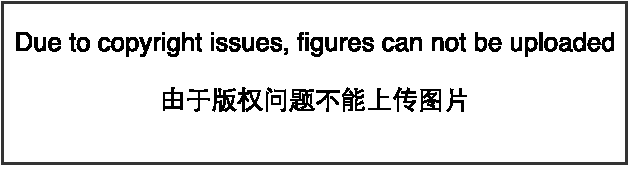
\includegraphics{figure.pdf}}
\else
\begin{tabular}{cc}
\includegraphics[width=0.4\textwidth]{Chapter11/figures/grid} &
\includegraphics[width=0.4\textwidth]{Chapter11/figures/random}
\end{tabular}
\fi
\caption{\gls{grid_search}和\gls{random_search}的比较。
为了方便地说明,我们只展示两个\gls{hyperparameter}的例子,但是通常我们关注的问题中\gls{hyperparameter}个数会更多。
(左)为了实现\gls{grid_search},我们为每个\gls{hyperparameter}提供了一个值的集合。
搜索算法对每一种在这些集合的交叉积中的\gls{hyperparameter}组合进行训练。
(右)为了实现\gls{random_search},我们给联合\gls{hyperparameter}赋予了一个概率分布。
通常\gls{hyperparameter}之间是相互独立的。
常见的这种分布的选择是均匀分布或者是对数均匀(从对数均匀分布中抽样,就是对从均匀分布中抽取的样本进行指数运算)的。
然后这些搜索算法联合的\gls{hyperparameter}空间中采样,然后运行每一个样本。
\gls{grid_search}和\gls{random_search}都运行了验证集上的误差并返回了最优的解。
这个图说明了通常只有一个\gls{hyperparameter}对结果有着重要的影响。
在这个例子中,只有水平轴上的\gls{hyperparameter}对结果有重要的作用。
\gls{grid_search}将大量的计算浪费在了指数级个数的对结果无影响的\gls{hyperparameter}中,相比之下\gls{random_search}几乎每次测试都测试了对结果有影响的每个\gls{hyperparameter}的一个值。
此图是从\citet{Bergstra+Bengio-LW2011}中复制的,并且经过了允许。}
\label{fig:chap11_grid_vs_random}
\end{figure}

应该如何选择搜索集合的范围呢?
在\gls{hyperparameter}是数值(有序)的情况下,每个列表的最小和最大的元素可以基于先前相似实验的经验保守地挑选出来,以确保最优解非常可能在所选范围内。
通常,\gls{grid_search}大约会在\firstgls{logarithmic_scale}下挑选合适的值,例如,一个学习率的取值集合是$\{0.1,0.01,10^{-3},10^{-4},10^{-5}\}$,或者\gls{hidden_unit}数目的取值集合$\{50,100,200,500,1000,2000\}$。

通常重复进行\gls{grid_search}时,效果会最好。
例如,假设我们在集合$\{-1,0,1\}$上\gls{grid_search}\gls{hyperparameter} $\alpha$。
如果找到的最佳值是$1$,那么说明我们低估了最优值$\alpha$所在的范围,应该扩大搜索范围,例如在集合$\{1,2,3\}$中搜索。
如果最佳值是$0$,那么我们不妨通过细化搜索范围以改进估计,在集合$\{-0.1,0,0.1\}$上进行\gls{grid_search}。

% -- 421 --

\gls{grid_search}带来的一个明显问题是,计算代价会随着\gls{hyperparameter}数量呈指数级增长。
如果有$m$个\gls{hyperparameter},每个至少取$n$个值,那么训练和估计所需的试验数将是$O(n^m)$。
可以并行地进行实验,并且并行要求十分宽松(不同搜索的机器之间几乎没有必要进行通信)。
令人遗憾的是,由于\gls{grid_search}指数级增长计算代价,即使是并行,我们也无法提供令人满意的计算能力。


\subsection{\glsentrytext{random_search}}
\label{sec:random_search}
幸运的是,有一个替代\gls{grid_search}的方法,并且编程简单,使用更方便,能更快地收敛到\gls{hyperparameter}的良好取值:\gls{random_search}\citep{Bergstra+Bengio-2012-small}。

\gls{random_search}过程如下。
首先,我们为每个\gls{hyperparameter}定义一个边缘分布,例如,\gls{bernoulli_distribution}或\gls{categorical_distribution}(对应着二元\gls{hyperparameter}或离散\gls{hyperparameter}),或者\gls{logarithmic_scale}上的均匀分布(对应着正实值\gls{hyperparameter})。
例如,
\begin{align}
	\texttt{log\_learning\_rate} &\sim u(-1, -5), \\
	\texttt{learning\_rate} &= 10^{\texttt{log\_learning\_rate}},
\end{align}
其中,$u(a,b)$表示区间$(a,b)$上均匀采样的样本。
类似地,$\texttt{log\_number\_of\_hidden\_units}$可能表示在$u(\log(50), \log(2000))$上采样。

和\gls{grid_search}不同,我们\emph{不需要离散化}\gls{hyperparameter}的值,我们可以在一个更大的集合上进行搜索,而不产生额外的计算代价。
实际上,如\figref{fig:chap11_grid_vs_random}所示,当有几个\gls{hyperparameter}对\gls{performance_metrics}没有很强的影响时,\gls{random_search}指数级高效于\gls{grid_search}。
\cite{Bergstra+Bengio-2012-small}进行了详细的研究,发现\gls{random_search}比\gls{grid_search}要快得多地减小验证集误差(就每个模型运行的试验数而言)。

与\gls{grid_search}一样,可以经常重复运行不同版本的\gls{random_search},以基于前一次运行的结果改进下一次搜索。

\gls{random_search}能比\gls{grid_search}更快地找到良好\gls{hyperparameter}的原因是,没有浪费的实验,不像\gls{grid_search}有时会对一个\gls{hyperparameter}的两个不同值(给定其他\gls{hyperparameter}值不变)给出相同结果。
在\gls{grid_search}中,其他\gls{hyperparameter}将在这两次实验中拥有相同的值,而在\gls{random_search}中,它们通常会具有不同的值。
因此,如果这两个值的变化不能勉强使验证集误差有明显区别的话,\gls{grid_search}没有必要重复两个等价的实验,而\gls{random_search}仍然会对其他\gls{hyperparameter}进行两次独立地探索。

% -- 422 --

\subsection{基于模型的\glsentrytext{hyperparameter}优化}
\label{sec:model_based_hyperparameter_optimization}
\gls{hyperparameter}搜索问题可以转化为一个优化问题。
决策变量是\gls{hyperparameter}。
优化的目标是最小化\gls{hyperparameter}训练出来的模型在\gls{validation_set}上的误差。
在简化的设定下,可以计算\gls{validation_set}上可导误差函数关于\gls{hyperparameter}的导数,然后我们遵循这个导数更新\citep{bengio:1999:snowbird,bengio-hyper-NC00,maclaurin2015gradient}。
令人遗憾的是,在大多数实际设定中,这个梯度是不可用的。
这可能是因为其高额的计算代价和存储成本,也可能是因为验证集误差在\gls{hyperparameter}上本质不可导,例如\gls{hyperparameter}是离散值的情况。

为了弥补导数这一不足,我们可以对验证集误差建模,然后通过优化该模型来提出新的\gls{hyperparameter}猜想。
大部分基于模型的\gls{hyperparameter}搜索算法,都是使用贝叶斯回归模型来估计每个\gls{hyperparameter}的验证集误差期望,和该期望的不确定性。
因此,优化涉及到探索(探索高度不确定的\gls{hyperparameter},可能有重大效果提升,也可能效果很差)和使用(使用已经确信效果不错的\gls{hyperparameter}——通常是先前非常熟悉的\gls{hyperparameter})之间的权衡。
关于\gls{hyperparameter}优化,现在的方法还有Spearmint\citep{Snoek+al-NIPS2012-small},TPE\citep{Bergstra+al-NIPS2011}和SMAC\citep{hutter+hoos+leyton+brown:2011}。

目前,我们无法明确确定,贝叶斯\gls{hyperparameter}优化是否是一个能够实现更好\gls{DL}结果或是能够事半功倍的工具。
贝叶斯\gls{hyperparameter}优化有时表现得像人类专家,能够在有些问题上取得很好的效果,但有时又会在某些问题上发生灾难性的失误。
看看它是否适用于一个特定的问题是值得尝试的,但目前该方法还不够成熟或可靠。
就像所说的那样,\gls{hyperparameter}优化是一个重要的研究领域,通常主要受\gls{DL}所需驱动,但是它不仅能贡献于整个\gls{ML}领域,还能贡献于一般的工程学。

% -- 423 --

大部分\gls{hyperparameter}优化算法比\gls{random_search}更复杂,并且具有一个共同的缺点,在它们能够从实验中提取任何信息之前,它们需要运行完整的训练实验。
相比于人类实践者手动搜索,考虑实验早期可以收集的信息量,这种方法是相当低效的,因为手动搜索通常可以很早判断出某组\gls{hyperparameter}是否是完全病态的。
\cite{swersky2014freeze}提出了一个可以维护多个实验的早期版本算法。
在不同的时间点,\gls{hyperparameter}优化算法可以选择开启一个新实验,``冻结''正在运行但希望不大的实验,或是``解冻''并恢复早期被冻结的,但现在根据更多信息后又有希望的实验。

\section{调试策略}
\label{sec:debugging_strategies}
当一个\gls{ML}系统效果不好时,通常很难判断效果不好的原因是算法本身,还是算法实现错误。
由于各种原因,\gls{ML}系统很难调试。

在大多数情况下,我们不能提前知道算法的预期行为。
事实上,使用\gls{ML}的整个出发点是,它会发现一些我们自己无法发现的有用行为。
如果我们在一个\emph{新}的分类任务上训练一个神经网络,它达到$5\%$的测试误差,我们没法直接知道这是期望的结果,还是次优的结果。

另一个难点是,大部分\gls{ML}模型有多个自适应的部分。
如果一个部分失效了,其他部分仍然可以自适应,并获得大致可接受的性能。
例如,假设我们正在训练多层神经网络,其中参数为权重$\MW$和\gls{bias_aff} $\Vb$。
进一步假设,我们单独手动实现了每个参数的梯度下降规则。
而我们在偏置更新时犯了一个错误:
\begin{equation}
	\Vb \leftarrow \Vb - \alpha,
\end{equation}
其中$\alpha$是学习率。
这个错误更新没有使用梯度。
它会导致偏置在整个学习中不断变为负值,而这显然是错误的。 
然而只是检查模型的输出,该错误可能并不是显而易见的。
根据输入的分布,权重可能可以自适应地补偿负的偏置。

% -- 424 --

大部分神经网络的调试策略都是解决这两个难题的一个或两个。
我们可以设计一种简单的情况,能够预见正确结果,判断和模型输出是否相符;我们也可以设计一个测试,检查神经网络实现的一部分。

一些重要的调试检测如下所列。

\emph{可视化模型的行为}:
当训练模型检测图像中的对象时,查看一些模型检测到部分重叠的图像。
在训练语音生成模型时,试听一些生成的语音样本。
这似乎是显而易见的,但在实际中很容易只注意量化\gls{performance_metrics},如\gls{accuracy}或对数似然。
直接观察\gls{ML}模型运行任务,有助于确定其达到的量化性能数据是否看上去合理。
错误评估模型性能可能是最具破坏性的错误之一,因为它们会使你在系统出问题时误以为系统运行良好。

\emph{可视化最严重的错误}:
大多数模型能够输出运行任务时的某种置信度量。
例如,基于\gls{softmax}输出层的分类器给每个类分配一个概率。
因此,分配给最有可能的类的概率给出了模型在其分类决定上的置信估计值。
通常,最大似然训练会高估正确预测的概率。
但是由于实际上模型的较小概率不太可能对应着正确的标签,因此它们在一定意义上还是有些用的。
通过查看训练集中很难正确建模的样本,通常可以发现该数据预处理或者标记方式的问题。
例如,街景\gls{transcription_system}原本有个问题是,地址号码检测系统会将图像裁剪得过于紧密,而省略掉了一些数字。
然后转录网络会分配非常低的概率给这些图像的正确答案。
将图像排序,确定置信度最高的错误,显示系统的裁剪有问题。
修改检测系统裁剪更宽的图像,从而使整个系统获得更好的性能,但是转录网络需要能够处理地址号码中位置和范围更大变化的情况。

\emph{根据训练和测试误差检测软件}:
往往很难确定底层软件是否是正确实现。
训练和测试误差能够提供一些线索。
如果训练误差较低,但是测试误差较高,那么很有可能训练过程是在正常运行,但模型由于算法原因过拟合了。
另一种可能是,测试误差没有被正确地度量,可能是由于训练后保存模型再重载去度量测试集时出现问题,或者是因为测试数据和训练数据预处理的方式不同。
如果训练和测试误差都很高,那么很难确定是软件错误,还是模型由于算法原因欠拟合。
这种情况需要进一步的测试,如下面所述。

% -- 425 --

\emph{拟合小数据集}:
当训练集上有很大的误差时,我们需要确定问题是欠拟合,还是软件错误。
通常,即使是小模型也可以保证很好地拟合一个足够小的数据集。
例如,只有一个样本的分类数据可以通过正确设置输出层的偏置来拟合。
通常,如果不能训练一个分类器来正确标注一个单独的样本,或不能训练一个\gls{AE}来成功地精准再现一个单独的样本,或不能训练一个生成模型来一致地生成一个单独的样本,那么很有可能是由于软件错误阻止训练集上的成功优化。
此测试可以扩展到只有少量样本的小数据集上。

\emph{比较反向传播导数和数值导数}:
如果正在使用一个需要实现梯度计算的软件框架,或者在添加一个新操作到求导库中,必须定义它的\texttt{bprop}方法,那么常见的错误原因是没能正确实现梯度表达。
验证这些求导正确的一种方法是比较实现的自动求导和\firstgls{finite_difference}计算的导数。
因为
\begin{equation}
	f'(x) = \lim_{\epsilon \to 0} \frac{f(x+\epsilon) - f(x)}{\epsilon},
\end{equation}
我们可以使用小的,有限的$\epsilon$近似导数:
\begin{equation}
	f'(x) \approx \frac{f(x+\epsilon) - f(x)}{\epsilon}.
\end{equation}
我们可以使用\firstgls{centered_difference}提高近似的\gls{accuracy}:
\begin{equation}
	f'(x) \approx \frac{ f(x+\frac{1}{2}\epsilon) - f(x-\frac{1}{2}\epsilon) }{\epsilon}.
\end{equation}
扰动大小$\epsilon$必须足够大,以确保该扰动不会由于数值计算的有限\gls{precision}问题向下近似太多。

% -- 426 --

通常,我们会测试向量值函数$g:\SetR^m \to \SetR^n$的梯度或\gls{jacobian}矩阵。
令人遗憾的是,\gls{finite_difference}只允许我们每次计算一个导数。
我们既可以运行\gls{finite_difference} $mn$次评估$g$的所有偏导数,又可以将该测试应用于一个输入输出都是$g$的随机投影的新函数。
例如,我们可以用导数实现去测试函数$f(x) = \Vu^T g(\Vv x)$,其中$\Vu$和$\Vv$是随机向量。
正确计算$f'(x)$要求能够正确地通过$g$反向传播,但是使用\gls{finite_difference}能够很有效地计算,因为$f$只有一个输入和一个输出。
在多个$\Vu$值和$\Vv$值上重复这个测试通常是个好主意,可以减少测试忽略了垂直于随机投影的几率。


如果可以在复数上进行数值计算,那么使用复数作为函数的输入能有非常高效的数值方法估算梯度\citep{Squire+Trapp-1998}。
该方法基于如下观察
\begin{align}
	f(x + i\epsilon) &= f(x) + i\epsilon f'(x) + O(\epsilon^2) ,\\
	\text{real}( f(x+i\epsilon) ) &= f(x) + O(\epsilon^2), \quad \text{image}( \frac{f(x+i\epsilon)}{ \epsilon } ) = f'(x) + O(\epsilon^2),
\end{align}
其中$i=\sqrt{-1}$。
和上面的实值情况不同,这里不存在$f$在不同点上计算差分消除影响。
因此我们可以使用很小的$\epsilon$,比如$\epsilon = 10^{-150}$,其中误差$O(\epsilon^2)$对所有实用目标都是微不足道的。


\emph{监控激励函数值和梯度的直方图}:
可视化神经网络在大量训练迭代后(也许是每个迭代)收集到的激励函数值和梯度的统计数据往往是有用的。
\gls{hidden_unit}的预激励值可以告诉我们该单元是否饱和,或者它们平常的状态如何。
例如,对于整流器,它们多久关一次?是否有单元一直关闭?
对于双曲正切单元而言,预激励绝对值的平均值可以告诉我们该单元的饱和程度。
在深度网络中,传播的梯度可以快速增长或快速消失,优化可能会受到阻碍。
最后,比较参数梯度和参数的量值也是有帮助的。
正如\citep{Bottou-DLSS2015}的建议,我们希望参数在一个\gls{minibatch}更新中变化的幅度是参数量值$1\%$这样的级别,而不是$50\%$或者$0.001\%$(这会导致参数移动得太慢)。
也有可能是某些参数以良好的步长移动,而另一些停滞。
如果数据是稀疏的(比如自然语言),有些参数可能很少更新,检测它们变化时应该记住这一点。

% -- 427 --

最后,许多\gls{DL}算法为每一步产生的结果提供了某种保证。
例如,在第三部分,我们将看到一些使用代数解决优化问题的近似推断算法。
通常,这些可以通过测试它们的每个担保来调试。
某些优化算法提供的保证包括,目标函数值在算法的迭代步中不会增加,某些变量的导数在算法的每一步中都是零,所有变量的导数都会收敛到零。
通常,由于舍入误差,这些条件不会在数字计算机上完全成立,因此调试测试应该包含一些允差参数。

\section{示例:多位数字识别}
\label{sec:example_multi_digit_number_recognition}
为了端到端地说明如何在实践中应用我们的设计方法,我们从\gls{DL}设计部分出发,简单地介绍下街景\gls{transcription_system}。
显然,整个系统的许多其他组件,如街景车,数据库设施,等等,也是极其重要的。

从\gls{ML}任务的视角出发,首先这个过程要采集数据。
街景车收集原始数据,然后操作员手动提供标签。
转录任务开始前有大量的数据处理工作,包括在转录前使用其他\gls{ML}技术\emph{探测}房屋号码。

转录项目开始于\gls{performance_metrics}的选择,和对这些度量的期望。
一个重要的总原则是度量的选择要符合项目的业务目标。
因为地图只有是高\gls{accuracy}时才有用,所以为这个项目设置高\gls{accuracy}的要求非常重要。
具体地,目标是达到人类水平,$98\%$的\gls{accuracy}。
这种程度的\gls{accuracy}并不是总能达到。
为了达到这个级别的\gls{accuracy},街景\gls{transcription_system}牺牲了\gls{coverage}。
因此在保持\gls{accuracy} $98\%$的情况下,\gls{coverage}成了这个项目优化的主要\gls{performance_metrics}。
随着卷积网络的改进,能够降低网络拒绝转录输入的置信度阈值,最终超出了\gls{coverage} $95\%$的目标。

% -- 428 --

在选择量化目标后,我们推荐方法的下一步是要快速建立一个合理的\gls{baseline}系统。
对于视觉任务而言,\gls{baseline}系统是带有\gls{ReLU}的\gls{convolutional_network}。
转录项目开始于一个这样的模型。
当时,使用卷积网络输出预测序列并不常见。
开始时,我们使用一个尽可能简单的\gls{baseline}模型,该模型输出层的第一个实现包含$n$个不同的\gls{softmax_unit}来预测$n$个字符的序列。
我们使用训练分类任务的方式来训练这些\gls{softmax_unit},单独训练每个\gls{softmax_unit}。


我们建议反复细化这些\gls{baseline},并测试每个变化是否都有改进。
街景\gls{transcription_system}的第一个变化受激励于\gls{coverage}指标的理论理解和数据的结构。
具体地,当输出序列的概率低于某个值$t$,$p(\Vy\mid\Vx) < t$时,网络拒绝为输入$\Vx$分类。
最初,$p(\Vy\mid\Vx)$的定义是临时的,简单地将所有\gls{softmax}输出乘在一起。
这促使我们后来发展能够真正计算出合理对数似然的特定输出层和损失函数。
这种方法使得样本拒绝机制发挥得更有效。


此时,\gls{coverage}仍低于$90\%$,但该方法没有明显的理论问题了。
因此,我们建议综合训练集和测试集性能,以确定问题是否是欠拟合或过拟合。
在这种情况下,训练和测试集误差几乎是一样的。
事实上,这个项目进行得如此顺利的主要原因是有数以千万计的标识样本数据集可用。
因为训练和测试集的误差是如此相似,这表明要么是这个问题欠拟合,要么是训练数据的问题。
我们推荐的调试策略之一是可视化模型最糟糕的错误。
在这种情况下,这意味着可视化不正确而模型给了最高置信度的训练集转录结果。
结果显示,主要是输入图像裁剪得太紧,有些和地址相关的数字被裁剪操作除去了。
例如,地址``1849''的图片可能裁切得太紧,只剩下``849''是可见的。
花费几周改进负责确定裁剪区域的地址号码检测系统的\gls{accuracy},或许可以解决这个问题。
与之不同,该项目团队采取了更实际的办法,简单地系统性扩大裁剪区域的宽度大于地址号码检测系统预测的区域。
这种单一改变给\gls{transcription_system}的\gls{coverage}增加了$10$个百分点。

% -- 429 --

最后,性能提升的最后几个百分点来自调整\gls{hyperparameter}。
这主要包括在保持一些计算代价限制的同时加大模型的规模。
因为训练误差和测试误差保持几乎相等,所以明确表明性能不足是由欠拟合造成的,数据集本身也存在一些问题。


总体来说,转录项目是非常成功的,可以比人工速度更快,代价更低地转录数以亿计的地址。

我们希望本章中介绍的设计原则能带来更多其他类似的成功。

% -- 430 --
